\chapter{The Transformer architecture}\label{ch:transformer-architecture}

\begin{chapterabstract}
    The Transformer is a unique ANN architecture researched at Google Brain and proposed in 2017 in the paper "Attention Is All You Need\cite{attention-is-all-you-need}."
    The model was a massive success in the natural language processing field.
    It was first designed for machine translation but has since been adapted to many other NLP tasks like text classification, text generation\cite{gpt1, gpt2, gpt3}, text summarization, question answering, and was even extended to work in computer vision\cite{dert, vision-transformer, image-transformer}.
\end{chapterabstract}


\section{Overview}\label{sec:overview}

The Transformer model takes advantage of an \textit{encoder-decoder} structure.
The encoder maps the input sequence $x = (x_1, \ldots, x_n)$ to a sequence of continuous representations $z = (z_1, \ldots, z_n)$.
We then pass representation $z$ to the decoder that generates the final output sequence $y = (y_1, \ldots, y_m)$ one symbol at a time.
At each step, the model is \textit{auto-regressive}, meaning it consumes previously generated symbols as additional input for the following step.
The Transformer implements this architecture using stacked point-wise, fully connected layers and self-attention for both the encoder and the decoder.
Please see the overall structure of the Transformer in figure~\ref{fig:transformer-overview}.~\cite{attention-is-all-you-need}


\begin{figure}
    \centering
    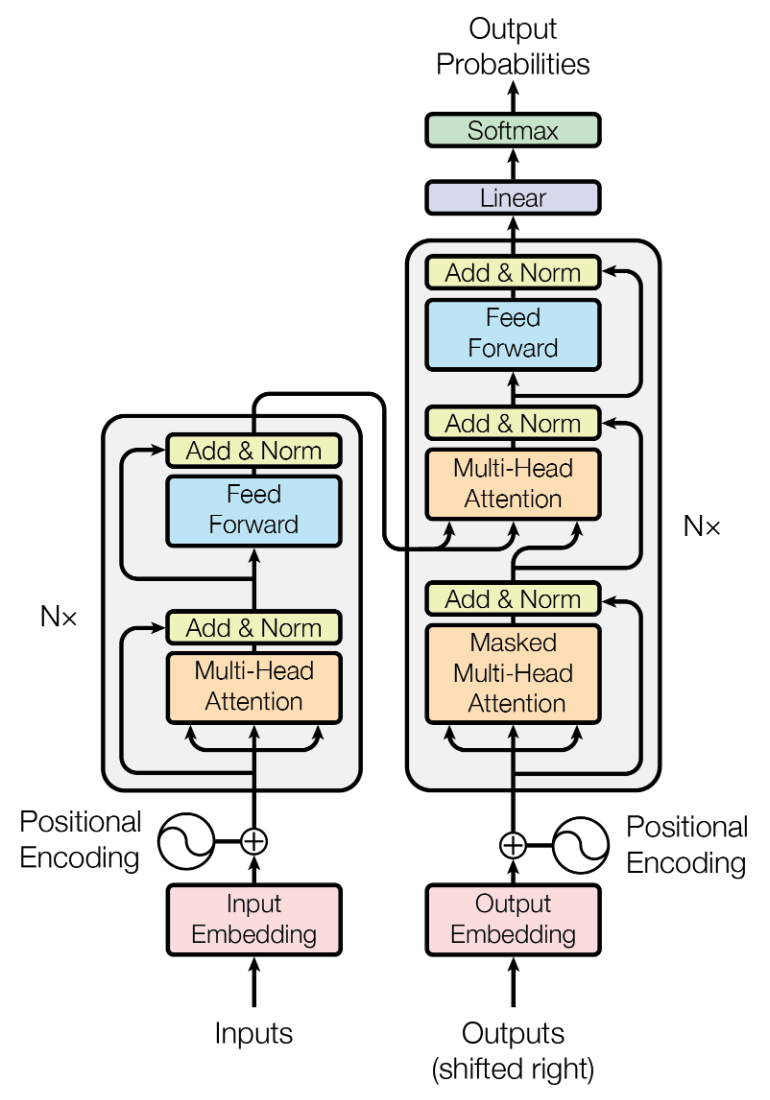
\includegraphics[width=0.6\textwidth]{assets/transformer-overview}
    \caption{~The Transformer - model architecture~\cite{attention-is-all-you-need}}\label{fig:transformer-overview}
\end{figure}


\section{Encoder}\label{sec:encoder}

The \textit{encoder} is formed of a stack of $N = 6$ identical layers.
Each layer has two sub-layers;
a \textit{multi-head self-attention} mechanism and a simple, position-wise, fully connected \textit{feed-forward network}.
The sub-layers use a \textit{residual connection}\footnote{residual connection means that not only consecutive layers are connected, but there are also additional connections bypassing a certain number of layers\cite{residual-connection}} around each of the two sub-layers, followed by layer normalization\cite{layer-normalization}.
To sum it up, the output of each sub-layer is $LayerNorm(x + Sublayer(x))$, where $Sublayer(x)$ is the function implemented by the sub-layer itself (self-attention/feed-forward ANN).
To enable these residual connections, all sub-layers in the model and the embedding layers produce outputs of dimension $d_{\text{model}} = 512$.
Visualization of the encoder module can be seen in figure~\ref{fig:encoder-decoder-detail}.~\cite{attention-is-all-you-need}


\begin{figure}
    \centering
    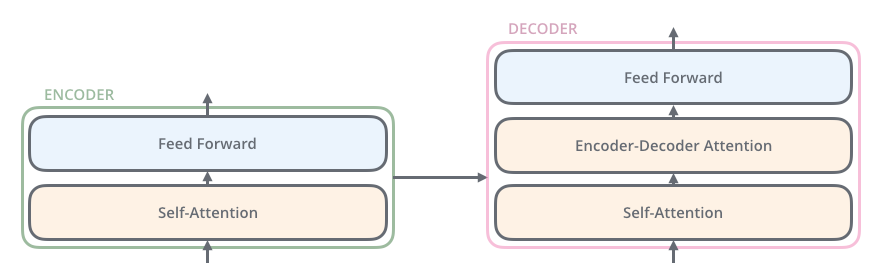
\includegraphics[width=0.86\textwidth]{assets/encoder-decoder-detail}
    \caption{~The encoder and decoder module detail~\cite{illustrated-transformer}}\label{fig:encoder-decoder-detail}
\end{figure}


\section{Decoder}\label{sec:decoder}


The \textit{decoder} comprises a stack of $N = 6$ identical layers as well.
The decoder module uses the same two sub-layers (just like the encoder) but, in addition to that, introduces a third sub-layer, which performs multi-head attention over the encoder's stack output.
Analogous to the encoder, we use layer normalization and residual connections when connecting sub-layers.
The \textit{self-attention} sub-layer in the decoder is modified to forbid positions from attending to successive positions.
Using this masking (also called teacher-forcing) and the fact that the output embeddings are shifted by one position ensures that predictions for an $i^{th}$ position depend exclusively on known positions less than $i$.~\cite{attention-is-all-you-need}
The decoder and its relation to the encoder can be seen in figure~\ref{fig:encoder-decoder-detail}.


\section{Attention}\label{sec:attention}

\textit{Attention} is the heart of the Transformer architecture;
it maps a \textit{query} and a set of \textit{key}-\textit{value} pairs to an output.
The output is computed as a sum weighted by a compatibility function of the query with the corresponding key.
The query, keys, and values are all represented as vectors.~\cite{attention-is-all-you-need}
The representation of attention can be seen in figure~\ref{fig:attention}.


\begin{figure}
    \centering
    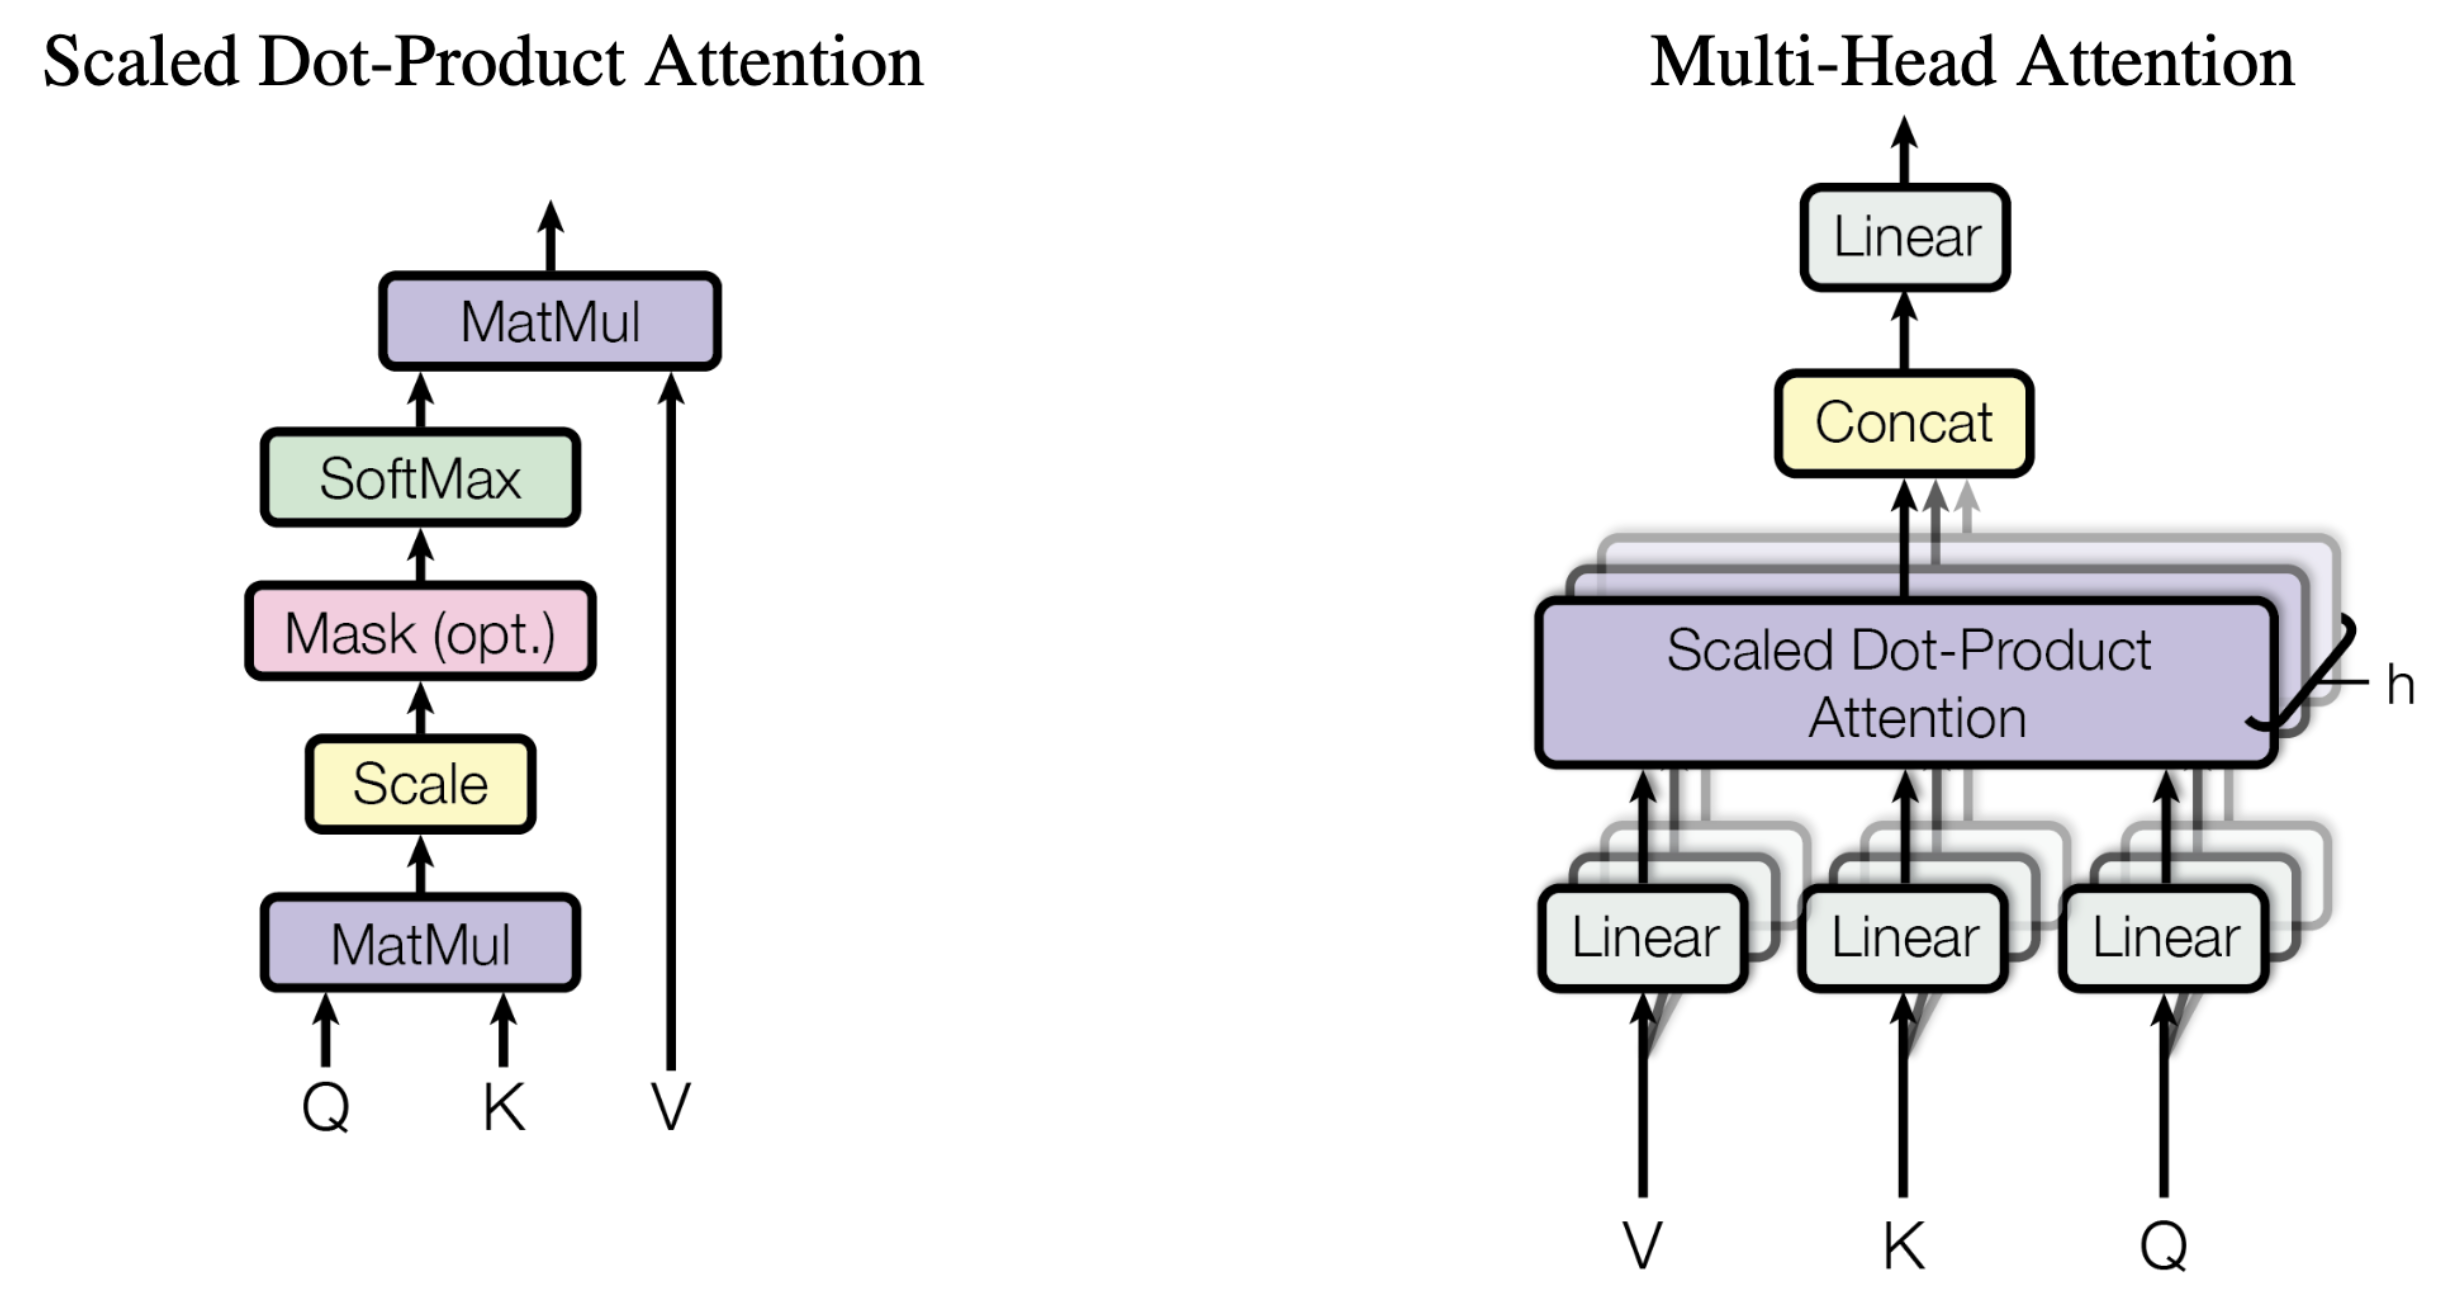
\includegraphics[width=\textwidth]{assets/attention}
    \caption{~Depiction of Scaled-Dot-Product Attention (left) and Multi-Head Attention (right)~\cite{attention-is-all-you-need}}\label{fig:attention}
\end{figure}

\subsection{Scaled Dot-Product Attention}\label{subsec:scaled-dot-product-attention}

The input for "Scaled Dot-Product Attention" consists of \textit{queries}, \textit{keys}, and \textit{values}.
The keys and queries take up dimension $d_k$, and the values take up dimension $d_v$.
The weights of values are computed by calculating the dot products of the query with all keys, each divided by $\sqrt{d_k}$, and finally, a \textit{softmax functio} is applied.
In practice, the attention function is computed on a set of queries, values, and keys simultaneously by packing them into \textit{matrices} \textbf{Q}, \textbf{K}, and \textbf{V}, respectively.~\cite{attention-is-all-you-need}
The matrix of outputs is computed as: \[ Attention(Q, K, V ) = softmax( \frac{QK^T}{\sqrt{d_k}}) V \]

The authors suspect that for large values of $d_k$, the dot products grow large in magnitude, pushing the softmax function into regions with minimal gradients.
Hence, to counteract this effect, the dot products are scaled by $\frac{1}{\sqrt{d_k}}$.~\cite{attention-is-all-you-need}

\subsection{Multi-Head Attention}\label{subsec:multi-head-attention}

The authors found that instead of using \textit{Scaled Dot-Product Attention} isolated, it is beneficial to \textit{linearly project} queries, keys, and values $h$ times with different learned linear projections to $d_k$, $d_k$, and $d_v$ dimensions.
The attention function is computed on all these projected versions of Q, K, and V in parallel, yielding $d_v$-dimensional output values.
Those are then concatenated and projected again, resulting in the final values.
Multi-head attention allows the model to attend to information from different representation subspaces at different positions at once.~\cite{attention-is-all-you-need}
Following is the formula for \textit{Multi-Head Attention}:

\begin{align*}
    MultiHead(Q, K, V) &= Concat(head_1, \ldots, head_h) W^O \\
    \text{where }head_i &= Attention(QW^Q_i, KW^K_i, VW^V_i)
\end{align*}

The projections are parameter matrices $W^Q_i \in \mathbb{R}^{d_{\text{model}} \times d_k}$, $W^K_i \in \mathbb{R}^{d_{\text{model}} \times d_k}$, $W^V_i \in \mathbb{R}^{d_{\text{model}} \times d_v}$, and $W^O \in \mathbb{R}^{hd_v \times d_{\text{model}}}$.

\subsection{Use of Attention inside the Transformer}\label{subsec:use-of-attention-inside-the-transformer}

Multi-head attention is used in three different places inside the Transformer.
The first occurrence is in the \textit{encoder-decoder layers}.
The queries come from the previous decoder layer, and keys and values come as outputs from the decoder.
Another way the multi-head attention is used is \textit{self-attention} (figure~\ref{fig:self-attention})), that is, when queries, keys, and values are all taken from the same place, in this case, from the output of the previous layer in the encoder.
The decoder also contains self-attention layers to allow all positions in the decoder to attend to any of the previous positions.
It must be prevented from attending a position that is after a given position to retain \textit{auto-regressivity}.
This is implemented inside the scaled dot-product attention by masking out all following values in the input.~\cite{attention-is-all-you-need}

\begin{figure}
    \centering
    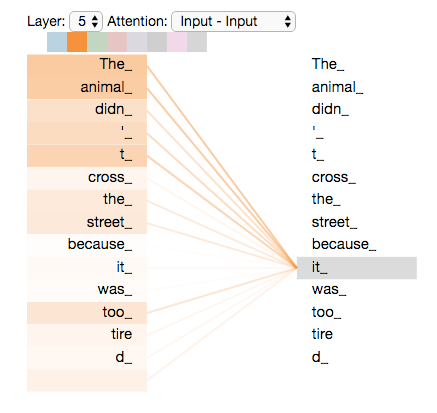
\includegraphics[width=0.5\textwidth]{assets/self-attention}
    \caption{~High-level depiction of self-Attention~\cite{illustrated-transformer}}\label{fig:self-attention}
\end{figure}


\section{Feed-forward networks}\label{sec:feed-forward-networks}

Aside from attention sub-layers, each layer in our encoder and decoder module contains a \textit{fully connected feed-forward} network applied to each position separately and identically~\cite{attention-is-all-you-need}.
The operation composes of two linear transformations with a ReLU activation in between:
\[
    \text{FFN}(x) = max(0, xW1 + b1)W2 + b2
\]
The input and output dimensions are $d_{model} = 512$, and the inner-layer has dimensionality $d_{ff} = 2048$~\cite{attention-is-all-you-need}.


\section{Embeddings and Softmax}\label{sec:embeddings-and-softmax}

The model uses learned \textit{embeddings}\footnote{\textit{``Embeddings are functions that map raw input data to low-dimensional vector representations, while preserving important semantic information about the inputs.''}\cite{embeddings}} to convert the input tokens and output tokens to vectors of the $d_{model}$ dimension.
The \textit{softmax function} converts the decoder output to predicted \textit{next token probabilities}.
The Transformer model shares the same weight matrix between the two embedding layers and the pre-softmax linear transformation.
The weights are then multiplied by $d_{model}$ in the embedding layers.~\cite{attention-is-all-you-need}


\section{Positional encoding}\label{sec:positional-encoding}

The model does not use any \textit{recurrent} or \textit{convolutional} layers, so for the model to understand the positions of all elements, we must provide additional information about the \textit{relative or absolute position} of the tokens in a sequence.
We add \textit{positional encodings} to the input embeddings at the bottoms of the encoder and decoder stacks to provide this information.
The positional encodings have the same dimension $d_{\text{model}}$ as the input embeddings to make summing possible.~\cite{attention-is-all-you-need}
Position encodings in the Transformer are calculated using the following formulas:
\begin{align*}
    PE(pos,2i) &= \sin (pos/10000^{2i/d_{\text{model}}}) \\
    PE(pos,2i+1) &= \cos (pos/10000^{2i/d_{\text{model}}})
\end{align*}
Where $i$ is the dimension and $pos$ is the position.
This results in each dimension of the positional encoding corresponding to a \textit{sinusoid}.
The \textit{wavelengths} create a geometric progression from $2\pi$ to $10000 \cdot 2\pi$.
The authors chose the sinusoidal version as they hypothesize it may allow the model to extrapolate to sequence lengths longer than the ones encountered during training.~\cite{attention-is-all-you-need}


\section{Music Transformer}\label{sec:music-transformer}

The Music Transformer is an \textit{auto-regressive} model based on the original Transformer.
A decoder-based\footnote{the encoder blocks from the original Transformer model are not used} model introduces modifications to the attention mechanism to enable \textit{relative} positional encoding and decrease memory requirements.~\cite{music-transformer}

\subsection{Relative positional encoding}\label{subsec:relative-positional-encoding}

\textit{``Music has multiple dimensions along which relative differences arguably matter more than their absolute values;
the two most prominent are timing and pitch.
To capture such pairwise relations between representations, Shaw et al.\cite{relative-positions} introduce a relation-aware version of self-attention which they use successfully to modulate self-attention by the distance between two positions.
We extend this approach to capture relative timing and''}~\cite{music-transformer}

Shaw et al.\cite{relative-positions} introduced \textit{relative position encoding} as an alternative to the Transformer's absolute position realized via positional sinusoids.
The relative positional encoding allows attention to be informed by how far two positions are apart in a given sequence.
This is done by training a separated relative position embedding $E^r$ of shape $(H, L, D_h)$, embedding every possible pairwise distance $r = j_k - i_q$ between a query and key in position $i_q$ and $j_k$, respectively.
The embeddings are then ordered by their distance from $-L + 1$ to $0$ (where $L$ means sequence length) and are learned separately for each head.
In the ``Self-attention with relative position representations,''\cite{relative-positions} the relative embeddings interact with queries and form a $S^{rel}$;
$L \times L$ dimensional logits\footnote{output layer values, before passed to softmax and becoming probabilities} matrix that modulates the attention probabilities for each head as follows\cite{music-transformer}:
\[
    \text{RelativeAttention} = \text{Softmax} \left( \frac{QK^T + S^{rel}}{sqrt{D_h}} \right) V
\]
The \textit{Music Transformer} uses the same approach to introduce \textit{relative distance} information to the attention computation while introducing a novel way of computing the $S^{rel}$, resulting in a significant memory footprint decrease.
In the ``Self-attention with relative position representations,''\cite{relative-positions} there is an intermediate tensor $R$ of shape $(L, L, D_h)$, instantiated for each head containing the embeddings corresponding to the relative distances between all keys and queries.
$Q$ is then reshaped to an $(L, 1, Dh)$ tensor and $S^{rel} = QR^T$.
This burdens the embedding computation to $O(L^2 D)$ space complexity, restricting use for longer sequences.~\cite{music-transformer}

\subsubsection{Efficient implementation}\label{subsubsec:efficient-implementation-of-relative-positional-encoding}

The Music Transformer improves the implementation of relative attention by reducing its \textit{intermediate memory} requirement from $O(L^2 D)$ to $O(LD)$.
The authors observed that all of the terms needed from $QR^T$ are already available by directly multiplying $Q$ with $Er$, the relative position embedding.
After the $QE^{rT}$ is computed, the $(i_q , r)$ entry contains the dot product of the query in position $i_q$ with the embedding of relative distance $r$.
Nevertheless, each relative logit $(i_q , j_k)$ in the matrix $S^{rel}$ from the previous equation should instead be the dot product of the query in position $i_q$ and the embedding of the relative distance $j_k - i_q$ , to match with the indexing in $QK^T$.
Therefore, we need to ``skew'' $QE^{rT}$ to move the relative logits to their correct positions, as is illustrated in figure~\ref{fig:rel-attention-skew}.
The time complexity for both methods is $O(L^2 D)$, but in practice, the authors report their method to be $6 \times$ faster at length $650$.~\cite{music-transformer}


\begin{figure}
    \centering
    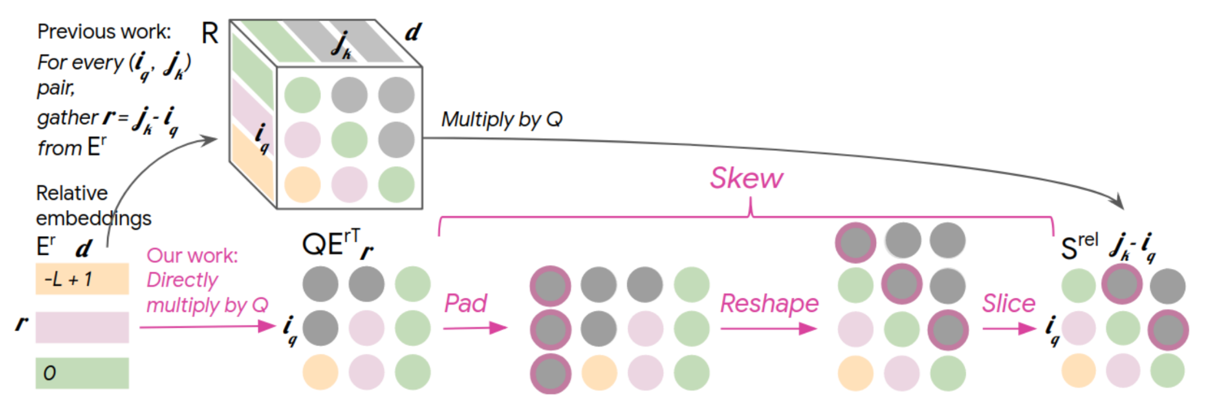
\includegraphics[width=\textwidth]{assets/rel-attention-skew}
    \caption{~Relative global attention: the bottom row describes the memory-efficient ``skewing'' algorithm. Gray indicates masked or padded positions. Each color corresponds to a different relative distance.~\cite{music-transformer}}\label{fig:rel-attention-skew}
\end{figure}

\subsection{Relative local attention}\label{subsec:relative-local-attention}

Local attention is not a new concept;
it has been used, for example, in Wikipedia and image generation\cite{sumarizing-wikipedia}.
It is realized by \textit{chunking} the input sequence into \textit{non-overlapping} blocks;
each block attends to itself and the one before, as shown by the smaller thumbnail on the top right corner of figure~\ref{fig:relative-local-attention}.
To extend the concept of relative attention to this local scope, we note that the right block has the same configuration as in the global case (see figure~\ref{fig:rel-attention-skew}) but smaller: $( \frac{L}{M} )^2$ (where $M$ refers the number of blocks, and $N$ be the resulting block length) instead of $L^2$.
The left block is unmasked with relative indices going from $-1$ (top right) to $-2N + 1$ (bottom left).
Because of that, the learned $E^r$ for the local scope has shape $(2N - 1, N)$.
Like the global case, we first compute $QE^{rT}$ and afterward use the following procedure to ``skew'' it to have the same indexing as $QK^T$>, as shown in figure~\ref{fig:relative-local-attention}.
The procedure is as follows\cite{music-transformer}:
\begin{enumerate}
    \item Pad dummy column vector with length $N$ after the rightmost column.
    \item Flatten the matrix and then pad with a dummy row having length $N - 1$.
    \item Reshape the matrix to the shape $(N + 1, 2N - 1)$.
    \item Slice obtained matrix to retain only the first $N$ rows and last $N$ columns, resulting in a matrix of shape $(N, N)$.
\end{enumerate}


\begin{figure}
    \centering
    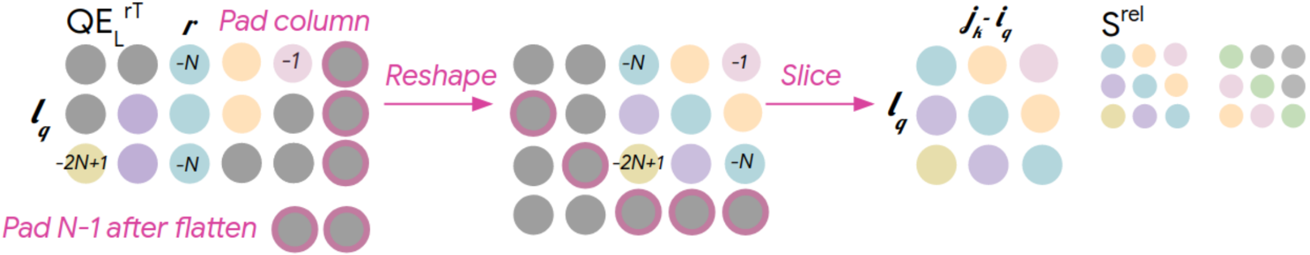
\includegraphics[width=\textwidth]{assets/relative-local-attention}
    \caption{~Relative local attention: the thumbnail on the right shows the desired configuration for $S^{rel}$. The ``skewing'' procedure is shown from left to right.~\cite{music-transformer}}\label{fig:relative-local-attention}
\end{figure}


